\documentclass[aps,onecolumn,twoside,secnumarabic,balancelastpage,amsmath,amssymb,nofootinbib,hyperref=pdftex]{revtex4}


\usepackage{color}         % produces boxes or entire pages with colored backgrounds
\usepackage{graphics}      % standard graphics specifications
\usepackage[pdftex]{graphicx}      % alternative graphics specifications
\usepackage{longtable}     % helps with long table options
\usepackage[english]{babel}
\setlength{\parskip}{1em}
\usepackage{amsmath}
\usepackage{epsf}          % old package handles encapsulated post script issues
\usepackage{bm}            % special 'bold-math' package
\usepackage{verbatim}			% for comment environment
\usepackage[colorlinks=true]{hyperref}  % this package should be added after all others % use as follows: \url{http://web.mit.edu/8.13}                                    
                                  

\begin{document}
\title{}
\author         {Noah Steinberg}
\email          {nastein@umich.edu}
\date{\today}
\affiliation{University of Michigan - Physics}

\maketitle

\section{Example: Running a BNV operator from below 10 TeV to 1 GeV }
In the Standard Model Effective Field Theory (SMEFT) there are four dimension six baryon number violating operators. In order to make predictions about proton decay rates or any other baryon number violating process, one must run the coefficients of these dimension six operators down to the scale where the physics process occurs, integrating out heavy particles as one passes through thresholds. We proceed with an example of this calculation below, utilizing two software packages: DSixTools\cite{DSixTools}, and RunDec\cite{RunDec}. DSixTools is used for running in the SMEFT, and RunDec is used for running in the Weak Effective Theory (WET). 
\newline

Consider the BNV dimension 6 operator $Q^{duql}_{prst} = C^{duql}_{prst}(\bar{d}^{c\alpha}_{p}u^{\beta}_{r})(\bar{q}^{ci\gamma}_{s}l^{j}_{t})\epsilon_{\alpha\beta\gamma}\epsilon_{ij}$, where i,j,k are $SU(2)_{L}$ indices, $\alpha$,$\beta$,$\gamma$ are SU(3) indices, and p,r,s,t are flavor indices.
\newline

RG equations for wilson coefficients in the SMEFT can be found in the appendix of DSixTools\cite{DSixTools}, we will not list them here. We will run down $C^{duql}_{1113}, C^{duql}_{1123}, C^{duql}_{1133}$, as these three coefficients will contribute to a single matched wilson coefficient in the WET. We arbitrarily set the value of these coefficients at $\mu = 10$ TeV to be $5\times10^{-5}$.
\newline

We run these coefficients down to $M_{\text{Top}}$ using DSixTools, the wilson coefficients each increase by $\approx 20$ percent from $\mu = 10$ TeV to $M_{\text{Top}}$.

\begin{figure}[htbp]
\begin{center}
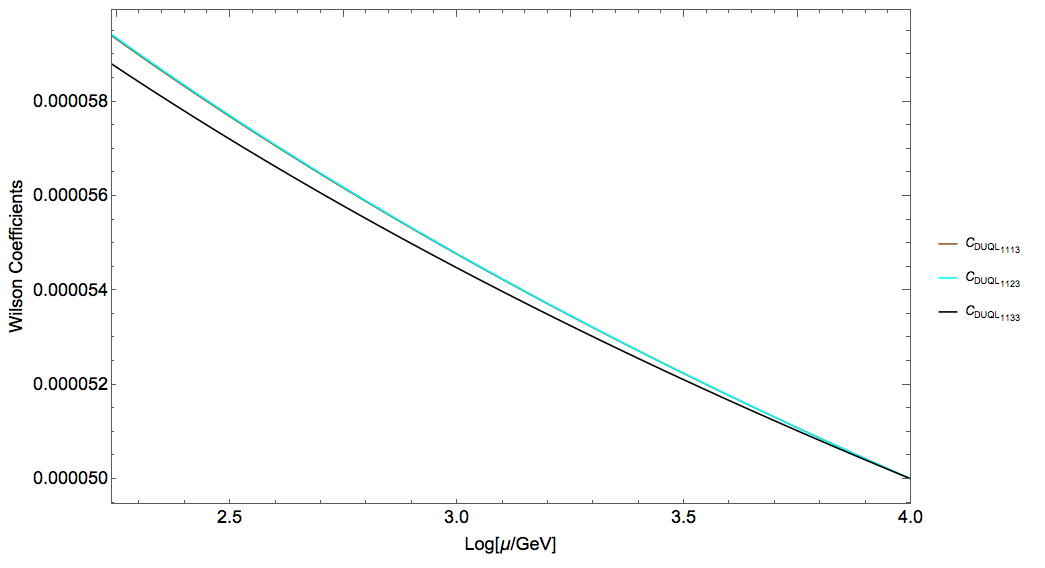
\includegraphics[width=10cm]{smeft_running.png}
\caption{Running of the three SMEFT wilson coefficients: $C^{duql}_{1113}(\mu), C^{duql}_{1123}(\mu), C^{duql}_{1133}(\mu)$ from 10 TeV to $M_{\text{Top}}$ using DSixTools.}
\label{default}
\end{center}
\end{figure}

Now we match the SMEFT to the WET where we have integrated out the top quark and broken electroweak symmetry. The SMEFT operators we considered above are matched to a single operator in the WET, $Q^{uds\nu_{\tau}}_{RL} = C^{uds\nu_{\tau}}_{RL}\epsilon_{\alpha\beta\gamma}(u^{\alpha}_{R}d^{\beta}_{R})(s^{\gamma}_{L}\nu_{\tau})$, with the matching condition

\begin{equation}
C^{uds\nu_{\tau}}_{RL}(M_{\text{Top}}) = -(V_{\text{CKM}})_{j2}C^{duql}_{11j3}(M_{\text{Top}})
\end{equation}

The above negative sign arises from contracting the SU(2) doublet index with the epsilon symbol. Using the above matching condition we can compute $C^{uds\nu_{\tau}}_{RL}(M_{\text{Top}}) = -7.361\times10^{-5}$. We then run down the wilson coefficient $C^{uds\nu_{\tau}}_{RL}(\mu)$ utilizing RunDec\cite{RunDec},  from $M_{\text{Top}}$ to 1 GeV. The two loop RG equation for the wilson coefficient $C(\mu)$ is given by 

\begin{equation}
\mu\frac{dC(\mu)}{d\mu} = -\left[4\frac{\alpha_{s}}{4\pi} + \left(\frac{14}{3} + \frac{4}{9}N_{f}  - \frac{10}{3}\right)\frac{\alpha_{s}^{2}}{(4\pi)^2}\right]C(\mu)
\end{equation}

Here we are only considering the QCD contribution to RG evolution in the WET because $\alpha_{s}$ is large. Using the two loop beta function for $\alpha_{s}$, we can write the solution for $C(\mu)$ as

\begin{equation}
\frac{C(\mu)}{C(\mu_0)} = \left[ \frac{\alpha_{s}(\mu)}{\alpha_{s}(\mu_0)}\right]^{-\frac{2}{b_1}}\left[ \frac{4\pi b_{1} + b_{2}\alpha_{s}(\mu)}{4\pi b_{1} + b_{2}\alpha_{s}(\mu_0)}\right]^{\frac{2}{b_1} - \frac{42 + 4N_{f}  + 9(-\frac{10}{3})}{18b_2}}
\end{equation}

where $b_1 = -\frac{11N_c - 2N_f}{3}$ and $b_2 = -\frac{34}{3}N^{2}_{c} + \frac{10}{3}N_{c}N_{f} + 2C_{F}N_{f}$. We can then calculate $C^{uds\nu_{\tau}}_{RL}(\mu)$ at any scale below $M_{\text{Top}}$ which we show below. 

\begin{figure}[htbp]
\begin{center}
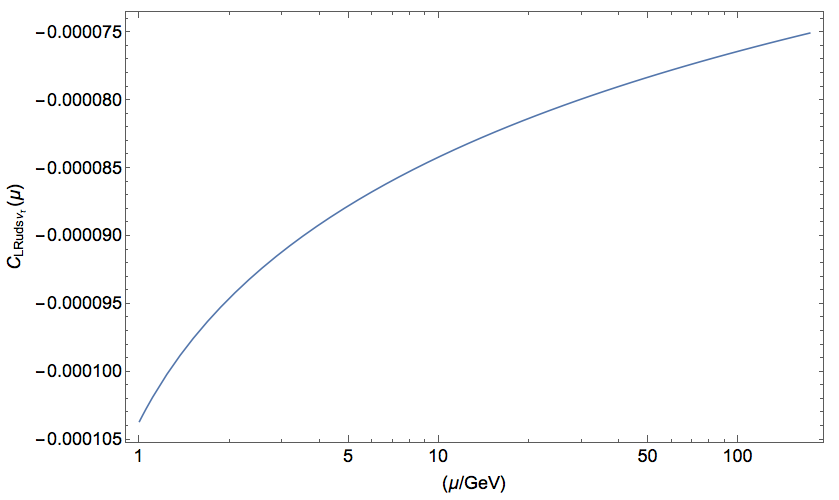
\includegraphics[width=10cm]{wet_running_1GeV.png}
\caption{Running of the WET wilson coefficient $C^{uds\nu_{\tau}}_{RL}(\mu)$ from $M_{\text{Top}}$ to 1 GeV}
\label{default}
\end{center}
\end{figure}

This gives $C^{uds\nu_{\tau}}_{RL}(\mu = 1 \text{GeV}) = -1.037\times10^{-4}$, this is a 41 percent increase in magnitude from $M_{\text{Top}}$ to 1 GeV. 

\begin{thebibliography}{9}

\bibitem{DSixTools} Celis, Alejandro et al., "DSixTools: The Standard Model Effective Field Theory Toolkit", arXiv:1704.04504 [hep-ph]
\bibitem{RunDec} Chetyrkin, K.G. et al., "RunDec: a Mathematica package for running and decoupling of the strong coupling and quark masses", arXiv:0004189 [hep-ph]

\end{thebibliography}

\end{document}